\documentclass[10pt]{scrartcl}

\usepackage[utf8]{inputenc}
\usepackage{tabularx}
\usepackage{longtable}
\usepackage[ngerman]{babel}
\usepackage[automark]{scrpage2}
\usepackage{amsmath,amssymb,amstext}
%\usepackage{mathtools}
\usepackage[]{color}
\usepackage[]{enumerate}
\usepackage{graphicx}
\usepackage{lastpage}
\usepackage[perpage,para,symbol*]{footmisc}
\usepackage{listings} 
\usepackage[pdfborder={0 0 0},colorlinks=false]{hyperref}
\usepackage[numbers,square]{natbib}
\usepackage{color}
\usepackage{colortbl}
\usepackage[absolute]{textpos}
\usepackage{float}
\usepackage[colorinlistoftodos,textsize=small,textwidth=2cm,shadow,bordercolor=black,backgroundcolor={red!100!green!33},linecolor=black]{todonotes}

\lstset{numbers=left, numberstyle=\tiny, numbersep=5pt, breaklines=true, showstringspaces=false} 
\restylefloat{figure}

%changehere
\def\titletext{Praktikum 1 : Stellen/Transitionsnetze}
\def\titletextshort{Praktikum 1}
\author{André Harms, Oliver Steenbuck}

\title{\titletext}

%changehere Datum der Übung
\date{06.06.2012}

\pagestyle{scrheadings}
%changehere
\ihead{TH1, Padberg}
\ifoot{Generiert am:\\ \today}


\cfoot{Oliver Steenbuck, André Harms}


\ohead[]{\titletextshort}
\ofoot[]{{\thepage} / \pageref{LastPage}}

\setlength{\parindent}{0.0in}
\setlength{\parskip}{0.1in}

\begin{document}
\maketitle

\setcounter{tocdepth}{3}
\tableofcontents

%	\listoftables                                 												% 
	\listoffigures  
%	\lstlistoflistings	

\section{Aufgabe 1}
	\subsection{Punkt 1}
				Kein Zusammenhang
				\begin{figure}[H]
    				\centering	
					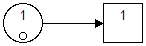
\includegraphics[scale=0.5]{aufg011.png}		
            		\caption{Lebendig, nicht reversibel}
				\end{figure}
				\begin{figure}[H]
    				\centering	
					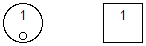
\includegraphics[scale=0.5]{aufg012.png}		
            		\caption{Nicht Lebendig, reversibel}
				\end{figure}
				\begin{figure}[H]
    				\centering	
					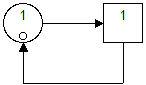
\includegraphics[scale=0.5]{aufg013.png}		
            		\caption{Lebendig, reversibel}
				\end{figure}
				\begin{figure}[H]
    				\centering	
					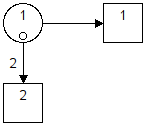
\includegraphics[scale=0.5]{aufg014.png}		
            		\caption{Nicht Lebendig, nicht reversibel}
				\end{figure}
				
	\subsection{Punkt 2}
	Kein Zusammenhang
				\begin{figure}[H]
    				\centering	
					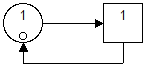
\includegraphics[scale=0.5]{aufg021.png}		
            		\caption{Lebendig, Beschränkt}
				\end{figure}
				\begin{figure}[H]
    				\centering	
					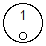
\includegraphics[scale=0.5]{aufg022.png}		
            		\caption{Nicht Lebendig, Beschränkt}
				\end{figure}
				\begin{figure}[H]
    				\centering	
					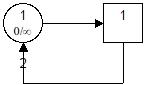
\includegraphics[scale=0.5]{aufg023.png}		
            		\caption{Lebendig, nicht Beschränkt}
				\end{figure}
				\begin{figure}[H]
    				\centering	
					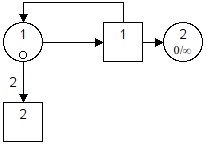
\includegraphics[scale=0.5]{aufg024.png}		
            		\caption{Nicht Lebendig, nicht Beschränkt}
				\end{figure}

		\subsection{Punkt 4}
		Sei Erreichbarkeit definiert als die Erreichbarkeit aller Markierungen in $N$ von $N_{M0}$ also $\forall M \in EG | M \textit{ ist Erreichbar von } N_{M0}$ dann gilt Lebendigkeit $\Longrightarrow$ Erreichbarkeit umgekehrt gilt dies nicht da für Erreichbarkeit nur der Hinweg gefordert ist.
		
		
		\subsection{Punkt 7}
		Kein Zusammenhang zwischen positiven Invarianten und Lebendigkeit.
				\begin{figure}[H]
    				\centering	
					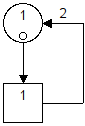
\includegraphics[scale=0.5]{aufg071.png}		
            		\caption{NichtInvariant, Lebendig}
				\end{figure}
				\begin{figure}[H]
    				\centering	
					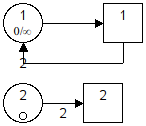
\includegraphics[scale=0.5]{aufg072.png}		
            		\caption{Nicht Invariant, Nicht Lebendig}
				\end{figure}
				\begin{figure}[H]
    				\centering	
					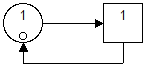
\includegraphics[scale=0.5]{aufg073.png}		
            		\caption{Invariant, Lebendig}
				\end{figure}
				\begin{figure}[H]
    				\centering	
					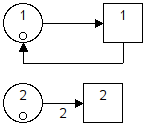
\includegraphics[scale=0.5]{aufg074.png}		
            		\caption{Invariant, Nicht Lebendig}
				\end{figure}
				
		\subsection{Punkt 11}
		Echt positive (alle Elemente positiv) T Invarianten $\Longleftrightarrow$ Lebendigkeit
		
		\subsection{Punkt 16}
		Sei $W_{all}(k)$ ein Weg der alle Knoten eines Graphen beinhaltet und bei $k$ startet und endet.
		So gilt $\forall u \in UG | \exists  W_{all}(u) \Longleftrightarrow \textit{Lebendigkeit}$		
		
		\subsection{Punkt 22}
		$|KG| = 1 \Longleftrightarrow Lebendigkeit$	
		
		\subsection{Punkt 29}
		Verklemmung $\Longrightarrow$ nicht Lebendig und Lebendig $\Longrightarrow$ keine Verklemmung.
		
		\subsection{Punkt 3}
		Kein Zusammenhang zwischen Beschränktheit und Reversibilität.
				\begin{figure}[H]
    				\centering	
					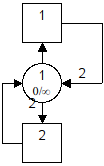
\includegraphics[scale=0.5]{aufg031.png}		
            		\caption{Nicht Beschränkt, Reversibel}
				\end{figure}
				\begin{figure}[H]
    				\centering	
					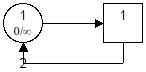
\includegraphics[scale=0.5]{aufg032.png}		
            		\caption{Nicht Beschränkt, Nicht Reversibel}
				\end{figure}
				\begin{figure}[H]
    				\centering	
					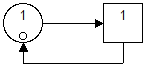
\includegraphics[scale=0.5]{aufg033.png}		
            		\caption{Beschränkt, Reversibel}
				\end{figure}
				\begin{figure}[H]
    				\centering	
					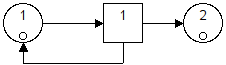
\includegraphics[scale=0.5]{aufg034.png}		
            		\caption{Beschränkt, Nicht Reversibel}
				\end{figure}
		
		
		\subsection{Punkt 5} 
		Reversibilität ist ein Spezialfall von Erreichbarkeit nämlich: $\forall m \in EG | M_0 \textit{ ist erreichbar}$
		
		\subsection{Punkt 8}
		Kein Zusammenhang zwischen P Invarianten und Reversibilität.
				\begin{figure}[H]
    				\centering	
					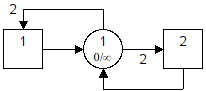
\includegraphics[scale=0.5]{aufg081.png}		
            		\caption{Nicht Invariant, Reversibel}
				\end{figure}
				\begin{figure}[H]
    				\centering	
					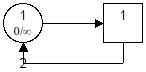
\includegraphics[scale=0.5]{aufg082.png}		
            		\caption{Nicht Invariant, Nicht Reversibel}
				\end{figure}
				\begin{figure}[H]
    				\centering	
					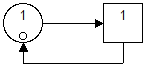
\includegraphics[scale=0.5]{aufg083.png}		
            		\caption{Invariant, Reversibel}
				\end{figure}
				\begin{figure}[H]
    				\centering	
					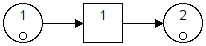
\includegraphics[scale=0.5]{aufg084.png}		
            		\caption{Invariant, Nicht Reversibel}
				\end{figure}
				
				\subsection{Punkt 12}
				Echt positive (alle Elemente positiv) T Invarianten $\Longleftrightarrow$ Reversibilität
				
				\subsection{Punkt 17}
				Sei $W_{all}(k)$ ein Weg der alle Knoten eines Graphen beinhaltet und bei $k$ startet und endet.
				So gilt $\forall u \in UG | \exists  W_{all}(u) \Longleftrightarrow \textit{Reversibilität}$	
				
				\subsection{Punkt 23}
				$|KG| = 1 \Longleftrightarrow \textit{Reversibilität}$ umgekehrt gilt dies nicht.
				
				
				\subsection{Punkt 30}
				Verklemmung $\Longrightarrow$ nicht Reversibel und Reversibel $\Longrightarrow$ keine Verklemmung.	
			
				\subsection{Punkt 6}
				Kein Zusammenhang zwischen Erreichbarkeit und Beschränktheit.
				\begin{figure}[H]
    				\centering	
					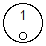
\includegraphics[scale=0.5]{aufg061.png}		
            		\caption{Nicht Erreichbar, Beschränkt}
				\end{figure}
				\begin{figure}[H]
    				\centering	
					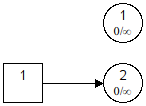
\includegraphics[scale=0.5]{aufg062.png}		
            		\caption{Nicht Erreichbar, Nicht Beschränkt}
				\end{figure}
				\begin{figure}[H]
    				\centering	
					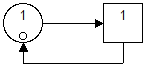
\includegraphics[scale=0.5]{aufg063.png}		
            		\caption{Erreichbar, Beschränkt}
				\end{figure}
				\begin{figure}[H]
    				\centering	
					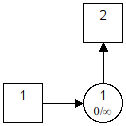
\includegraphics[scale=0.5]{aufg064.png}		
            		\caption{Erreichbar, Nicht Beschränkt}
				\end{figure}		
				
				
				\subsection{Punkt 9}
				Echt positive (alle Elemente positiv) P Invarianten $\Longleftrightarrow$ Beschränktheit.
				
				 \subsection{Punkt 13}
				 Es gibt keinen Zusammenhang zwischen echt positiven T Invarianten und der Beschränktheit eines Netzes.
				 \begin{figure}[H]
    				\centering	
					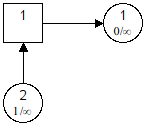
\includegraphics[scale=0.5]{aufg0131.png}		
            		\caption{Nicht Invariant, Beschränkt}
				\end{figure}
				\begin{figure}[H]
    				\centering	
					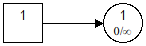
\includegraphics[scale=0.5]{aufg0132.png}		
            		\caption{Nicht Invariant, Nicht Beschränkt}
				\end{figure}
				\begin{figure}[H]
    				\centering	
					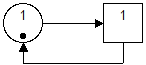
\includegraphics[scale=0.5]{aufg0133.png}		
            		\caption{Invariant, Beschränkt}
				\end{figure}
				\begin{figure}[H]
    				\centering	
					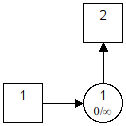
\includegraphics[scale=0.5]{aufg0134.png}		
            		\caption{Invariant, Nicht Beschränkt}
				\end{figure}
				 
			\subsection{Punkt 18}
			Überdeckungsgraph ohne $\omega$ $\Longleftrightarrow$ Beschränktheit 	 
			
			\subsection{Punkt 24}	
			Es besteht kein Zusammenhang zwischen der Größe des Kondensationsgraphen und der Beschränkheit des Netzes.	
			\begin{figure}[H]
    				\centering	
					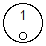
\includegraphics[scale=0.5]{aufg0241.png}		
            		\caption{KG 1 Knoten, Beschränkt}
				\end{figure}
				\begin{figure}[H]
    				\centering	
					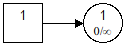
\includegraphics[scale=0.5]{aufg0242.png}		
            		\caption{KG 1 Knoten, Nicht Beschränkt}
				\end{figure}
				\begin{figure}[H]
    				\centering	
					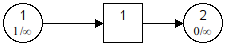
\includegraphics[scale=0.5]{aufg0243.png}		
            		\caption{KG 2 Knoten, Beschränkt}
				\end{figure}
				\begin{figure}[H]
    				\centering	
					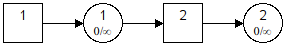
\includegraphics[scale=0.5]{aufg0244.png}		
            		\caption{KG 2 Knoten, Nicht Beschränkt}
				\end{figure}	
				
				\subsection{Punkt 31}
				Verklemmung $\Longrightarrow$ Beschränktheit
			
				\subsection{Punkt 10}
				Wir sehen keinen Zusammenhang, die Konzepte wirken komplett losgelöst voneinander.
				
				\subsection{Punkt 14}	
				Positive T Invarianten $\Longrightarrow$ Erreichbarkeit der positiven auftretenden Transisitionen. 
				
				\subsection{Punkt 19}
				Ein Überdeckungsgraph ist eine mögliche endliche graphische Abbildung der Erreichbarkeitseigenschaften eines Netzes.
				
				\subsection{Punkt 25}
				$|KG| = 1 \Longleftrightarrow \forall m \in EG | \text{m ist Erreichbar}$ 
			
				\subsection{Punkt 32}
				$\forall t  \in T \textbf{ } \neg \exists m \in M | \text{ t ist M-erreichbar aus m } \Longrightarrow \text{Verklemmung} $\\ oder: Wenn keine Transision aus $m$ Erreichbar ist dann ist das Netz unter $m$ Verklemmt.
				
				\subsection{Punkt 15}
				Die T Invarianten eines Netzes S/T $N$ sind die P Invarianten des dualen Netzes $dual(N)$
				
				\subsection{Punkt 20}
				Eine komplett positive P Invariante $\Longrightarrow$ Keine $\omega$ im UG
				
				\subsection{Punkt 26}
				Kondensationsgraph und komplett positive Stelleninvarianten besitzen keinen Zusammenhang
				\begin{figure}[H]
    				\centering	
					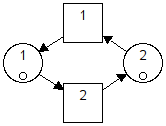
\includegraphics[scale=0.5]{aufg0261.png}		
            		\caption{KG 1 Knoten, Invariant}
				\end{figure}
				\begin{figure}[H]
    				\centering	
					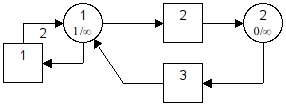
\includegraphics[scale=0.5]{aufg0262.png}		
            		\caption{KG 1 Knoten, Nicht Invariant}
				\end{figure}
				\begin{figure}[H]
    				\centering	
					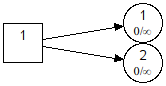
\includegraphics[scale=0.5]{aufg0263.png}		
            		\caption{KG 2 Knoten, Invariant}
				\end{figure}
				\begin{figure}[H]
    				\centering	
					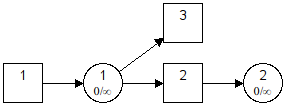
\includegraphics[scale=0.5]{aufg0264.png}		
            		\caption{KG 2 Knoten, Nicht Invariant}
				\end{figure}
				
				\subsection{Punkt 33}
				Die Verklemmung von $M_0$ impliziert das Vorhandensein einer P Invariante in der alle Stellen mit $1$ gewichtet werden.
				
				\subsection{Punkt 21}
				$\omega$ freie Zyklen im Überdeckungsgraphen $\Longrightarrow$ T Invarianten der im Zyklus genutzten Transitionen.
				
				\subsection{Punkt 27}
				$|KG| = 1 \Longrightarrow $ es existiert eine komplett positive T Invariante.
				
				\subsection{Punkt 34}
				Die komplett positive T Invariante $\Longrightarrow$ keine Verklemmung
				
				\subsection{Punkt 28}
				Der KG bildet die stark zusammenhängenen Knoten im Überdeckungsgraphen ab.
				
				\subsection{Punkt 35}
				Keine Senken im Überdeckungsgraphen $\Longrightarrow$ keine Verklemmungen
				
				\subsection{Punkt 36}
				$|KG| = 1 \Longrightarrow $ keine Verklemmung 
				
				\section{Aufgabe 2}
				Folgende Konzepte bilden in unseren Augen Teile der Korrektheitseigenschaften des Protokolls.
				\subsection{Lebendigkeit}
				Es sollte im Protokoll für einen von beiden Teilnehmer immer möglich sein Nachrichten zu versenden.
				
				\subsection{Reversibilität}
				Wenn alle Nachrichten angekommen sind sollte sich das Protokoll wieder im Ursprungszustand befinden.
				
				\subsection{Verklemmung}
				Das Protokoll darf keine Verklemmungen beinhalten, da es keine Deadlocks vorsieht.
				
				\subsection{Kondesationgraph}
				Der Kondensationsgraph muß die Mächtigkeit 1 haben da von jedem Zustand jeder andere Zustand Erreichbar ist.
				
				\subsection{Nachweisbarkeit}
				Wir würden mit der Konstruktion des KG beginnen um über diesen Nachzuweisen das er die Mächtigkeit 1 hat und es daher keine Verklemmungen geben kann sowie das das Netz Reversibel und Lebendig ist.
								
				
\end{document}

